% GNUPLOT: LaTeX picture with Postscript
\begingroup
  \makeatletter
  \providecommand\color[2][]{%
    \GenericError{(gnuplot) \space\space\space\@spaces}{%
      Package color not loaded in conjunction with
      terminal option `colourtext'%
    }{See the gnuplot documentation for explanation.%
    }{Either use 'blacktext' in gnuplot or load the package
      color.sty in LaTeX.}%
    \renewcommand\color[2][]{}%
  }%
  \providecommand\includegraphics[2][]{%
    \GenericError{(gnuplot) \space\space\space\@spaces}{%
      Package graphicx or graphics not loaded%
    }{See the gnuplot documentation for explanation.%
    }{The gnuplot epslatex terminal needs graphicx.sty or graphics.sty.}%
    \renewcommand\includegraphics[2][]{}%
  }%
  \providecommand\rotatebox[2]{#2}%
  \@ifundefined{ifGPcolor}{%
    \newif\ifGPcolor
    \GPcolortrue
  }{}%
  \@ifundefined{ifGPblacktext}{%
    \newif\ifGPblacktext
    \GPblacktexttrue
  }{}%
  % define a \g@addto@macro without @ in the name:
  \let\gplgaddtomacro\g@addto@macro
  % define empty templates for all commands taking text:
  \gdef\gplbacktext{}%
  \gdef\gplfronttext{}%
  \makeatother
  \ifGPblacktext
    % no textcolor at all
    \def\colorrgb#1{}%
    \def\colorgray#1{}%
  \else
    % gray or color?
    \ifGPcolor
      \def\colorrgb#1{\color[rgb]{#1}}%
      \def\colorgray#1{\color[gray]{#1}}%
      \expandafter\def\csname LTw\endcsname{\color{white}}%
      \expandafter\def\csname LTb\endcsname{\color{black}}%
      \expandafter\def\csname LTa\endcsname{\color{black}}%
      \expandafter\def\csname LT0\endcsname{\color[rgb]{1,0,0}}%
      \expandafter\def\csname LT1\endcsname{\color[rgb]{0,1,0}}%
      \expandafter\def\csname LT2\endcsname{\color[rgb]{0,0,1}}%
      \expandafter\def\csname LT3\endcsname{\color[rgb]{1,0,1}}%
      \expandafter\def\csname LT4\endcsname{\color[rgb]{0,1,1}}%
      \expandafter\def\csname LT5\endcsname{\color[rgb]{1,1,0}}%
      \expandafter\def\csname LT6\endcsname{\color[rgb]{0,0,0}}%
      \expandafter\def\csname LT7\endcsname{\color[rgb]{1,0.3,0}}%
      \expandafter\def\csname LT8\endcsname{\color[rgb]{0.5,0.5,0.5}}%
    \else
      % gray
      \def\colorrgb#1{\color{black}}%
      \def\colorgray#1{\color[gray]{#1}}%
      \expandafter\def\csname LTw\endcsname{\color{white}}%
      \expandafter\def\csname LTb\endcsname{\color{black}}%
      \expandafter\def\csname LTa\endcsname{\color{black}}%
      \expandafter\def\csname LT0\endcsname{\color{black}}%
      \expandafter\def\csname LT1\endcsname{\color{black}}%
      \expandafter\def\csname LT2\endcsname{\color{black}}%
      \expandafter\def\csname LT3\endcsname{\color{black}}%
      \expandafter\def\csname LT4\endcsname{\color{black}}%
      \expandafter\def\csname LT5\endcsname{\color{black}}%
      \expandafter\def\csname LT6\endcsname{\color{black}}%
      \expandafter\def\csname LT7\endcsname{\color{black}}%
      \expandafter\def\csname LT8\endcsname{\color{black}}%
    \fi
  \fi
  \setlength{\unitlength}{0.0500bp}%
  \begin{picture}(8502.00,6802.00)%
    \gplgaddtomacro\gplbacktext{%
      \csname LTb\endcsname%
      \put(592,2139){\makebox(0,0)[r]{\strut{} 51}}%
      \csname LTb\endcsname%
      \put(592,3256){\makebox(0,0)[r]{\strut{} 54}}%
      \csname LTb\endcsname%
      \put(592,4374){\makebox(0,0)[r]{\strut{} 57}}%
      \csname LTb\endcsname%
      \put(592,5491){\makebox(0,0)[r]{\strut{} 60}}%
      \csname LTb\endcsname%
      \put(592,6609){\makebox(0,0)[r]{\strut{} 63}}%
      \csname LTb\endcsname%
      \put(688,1408){\rotatebox{-270}{\makebox(0,0)[r]{\strut{}lrelu001}}}%
      \csname LTb\endcsname%
      \put(1158,1408){\rotatebox{-270}{\makebox(0,0)[r]{\strut{}relu}}}%
      \csname LTb\endcsname%
      \put(1627,1408){\rotatebox{-270}{\makebox(0,0)[r]{\strut{}swish}}}%
      \csname LTb\endcsname%
      \put(2097,1408){\rotatebox{-270}{\makebox(0,0)[r]{\strut{}penalized\_tanh}}}%
      \csname LTb\endcsname%
      \put(2567,1408){\rotatebox{-270}{\makebox(0,0)[r]{\strut{}lrelu030}}}%
      \csname LTb\endcsname%
      \put(3036,1408){\rotatebox{-270}{\makebox(0,0)[r]{\strut{}tanhrev}}}%
      \csname LTb\endcsname%
      \put(3506,1408){\rotatebox{-270}{\makebox(0,0)[r]{\strut{}elu}}}%
      \csname LTb\endcsname%
      \put(3976,1408){\rotatebox{-270}{\makebox(0,0)[r]{\strut{}minsin}}}%
      \csname LTb\endcsname%
      \put(4445,1408){\rotatebox{-270}{\makebox(0,0)[r]{\strut{}maxtanh}}}%
      \csname LTb\endcsname%
      \put(4915,1408){\rotatebox{-270}{\makebox(0,0)[r]{\strut{}tanh}}}%
      \csname LTb\endcsname%
      \put(5385,1408){\rotatebox{-270}{\makebox(0,0)[r]{\strut{}sin}}}%
      \csname LTb\endcsname%
      \put(5854,1408){\rotatebox{-270}{\makebox(0,0)[r]{\strut{}maxsig}}}%
      \csname LTb\endcsname%
      \put(6324,1408){\rotatebox{-270}{\makebox(0,0)[r]{\strut{}selu}}}%
      \csname LTb\endcsname%
      \put(6794,1408){\rotatebox{-270}{\makebox(0,0)[r]{\strut{}linear}}}%
      \csname LTb\endcsname%
      \put(7263,1408){\rotatebox{-270}{\makebox(0,0)[r]{\strut{}sigmoid}}}%
      \csname LTb\endcsname%
      \put(7733,1408){\rotatebox{-270}{\makebox(0,0)[r]{\strut{}cosper}}}%
      \put(7829,2818){\makebox(0,0)[l]{\strut{} 18}}%
      \put(7829,3679){\makebox(0,0)[l]{\strut{} 23}}%
      \put(7829,4541){\makebox(0,0)[l]{\strut{} 28}}%
      \put(7829,5403){\makebox(0,0)[l]{\strut{} 33}}%
      \put(7829,6264){\makebox(0,0)[l]{\strut{} 38}}%
      \put(128,4056){\rotatebox{-270}{\makebox(0,0){\strut{}Score}}}%
    }%
    \gplgaddtomacro\gplfronttext{%
      \csname LTb\endcsname%
      \put(6998,6466){\makebox(0,0)[r]{\strut{}Best}}%
      \csname LTb\endcsname%
      \put(6998,6306){\makebox(0,0)[r]{\strut{}Avg}}%
    }%
    \gplbacktext
    \put(0,0){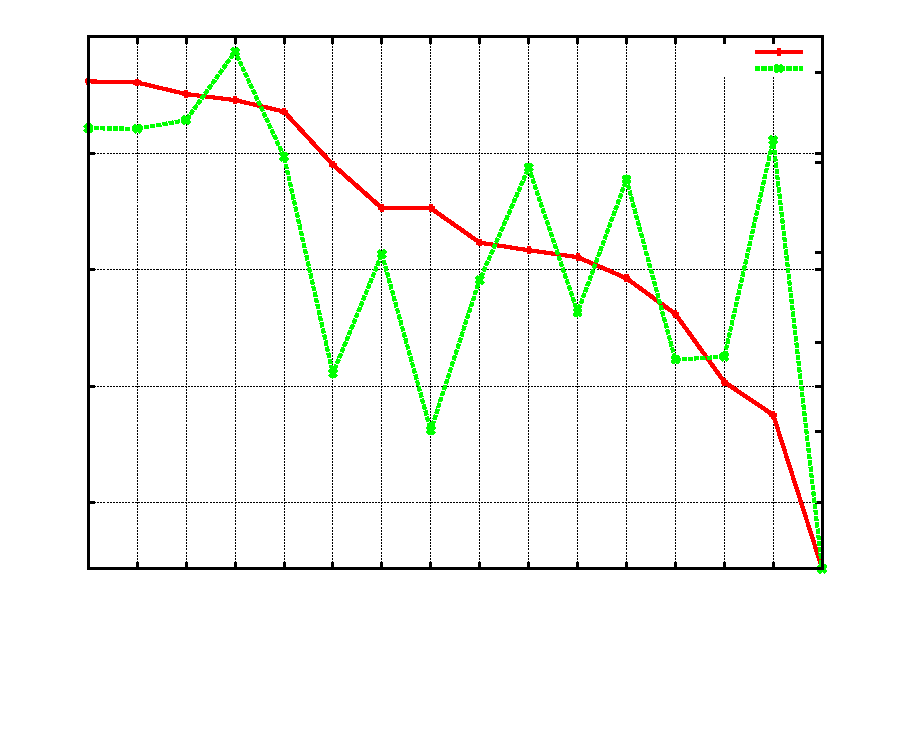
\includegraphics{plots/seq2}}%
    \gplfronttext
  \end{picture}%
\endgroup
